\documentclass[11pt]{amsart}
\usepackage[utf8]{inputenc}
\usepackage[english]{babel}
\usepackage{amsmath}
\usepackage{amsfonts}
\usepackage{amssymb}
\usepackage[all]{xy}
\usepackage{graphicx}

\begin{document}

\title{Modelling Stochastic Time Delay Structures for Regression}
\author{Aaron Pickering}
%\address{}
\email{aaron1rcl@gmail.com}
%\urladdr{} 
\date{\today}
\maketitle

\section{Introduction}

Consider the typical univariate regression problem where the intention is to find
the relationship between $x$ and $y$. When extended to time series, a number of time specific complexities arise. For the specific case where the input $x$ affects the output $y$, with a random time delay in between, the estimated coefficients (or weights, predictions etc) are significantly attenuated. This attenuation occurs both in traditional statistical models and machine learning models, and for certain problems can be a serious limitation. The following document proposes techniques for handling this class of time series regression.

As an example, let us take the management of blood sugar level in diabetes patients. In people with diabetes, the pancreas can't effectively regulate blood sugar levels. Therefore, these levels must be controlled by insulin injections and a special diet. The challenge for many people is that the relationship between the input (insulin) and output (blood sugar) is extremely complex. The effect of the insulin injection might be observed after $15$, $20$  or $t$ minutes depending on a number of factors, many of which are unknown. Due to the stochastic nature of the time delays, the actual effect can't be easily determined. It is difficult to differentiate the effect of the insulin injection from other factors and accurately determine how much one should take.

Inference for this type of problem is especially challenging. Typical regression models require a fixed alignment between cause and effect. Using standard methods, we'd need to assume that the effect occurs after some fixed time 't' which can be inferred from the data. However, if there is any uncertainty in the parameter $t$ ($t$ changes or is noisy) the resulting estimates will be significantly attenuated.

Consider the simple example where the effect of the input is $1$, as shown in the image below. The observed input is given by the red line, the blue line is when the effect actually occurs. The first effect happens 1 time point after the input. The second effect happens at the same time as the input. A fixed time delay isn't valid in this case because the time shifts differ.

\begin{center}
\begin{figure}
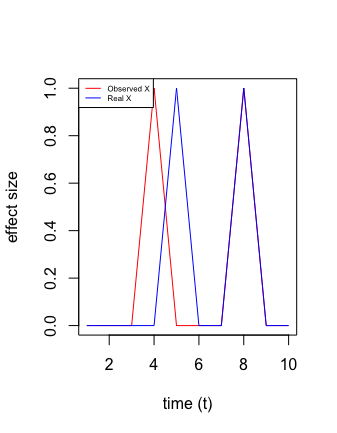
\includegraphics[totalheight=8cm]{images/1_input_delay_example.png}
\caption{Add figure caption}
\label{fig:verticalcell}
\end{figure}
\end{center}

If one were to model the effect using a fixed time delay and OLS, the estimate would only be half the true value because only one of the outputs is aligned. Obviously, this isn't ideal, we want the parameter estimates to be as close to the real values as possible, regardless of any noise in the lag structures. One can mitigate the problem via time aggregations, however in complicated multivariate cases, this is just not feasible.

Therefore, we propose a regression model which can handle stochastic time delay structures. We treat the stochastic time delay components as an ‘error’ in the time axis. Next, we find the maximum likelihood estimate, for a given set of parameters, considering the time error ($t$-axis) and the regression error ($y$-axis) simultaneously.


\section{Methodology}

...





\end{document}